\documentclass[tikz,border=2pt]{standalone}
\usepackage{lmodern}
\usepackage[T1]{fontenc}
\usepackage{amsmath,amssymb}
\newcommand{\ee}{\mathrm{e}}
\newcommand{\ii}{\mathrm{i}}
\usetikzlibrary{arrows.meta,calc,decorations.markings}

% Keep script and scriptscript at the 8 pt print floor (column scale ~1).
\DeclareMathSizes{8}{8}{8}{8}
\DeclareMathSizes{9}{9}{8}{8}

\definecolor{brownpop}{HTML}{D55E00}
\definecolor{tealpop}{HTML}{0072B2}
\definecolor{ink}{HTML}{222222}
\definecolor{muted}{HTML}{555555}
\definecolor{patch}{HTML}{E69F00}
\definecolor{boxfill}{HTML}{F4F7FA}
\definecolor{boxedge}{HTML}{C5CDD4}
\definecolor{gramfill}{HTML}{D9DEE3}
\definecolor{blockfill}{HTML}{E6E8EB}
\definecolor{blockedge}{HTML}{6B7280}

\begin{document}
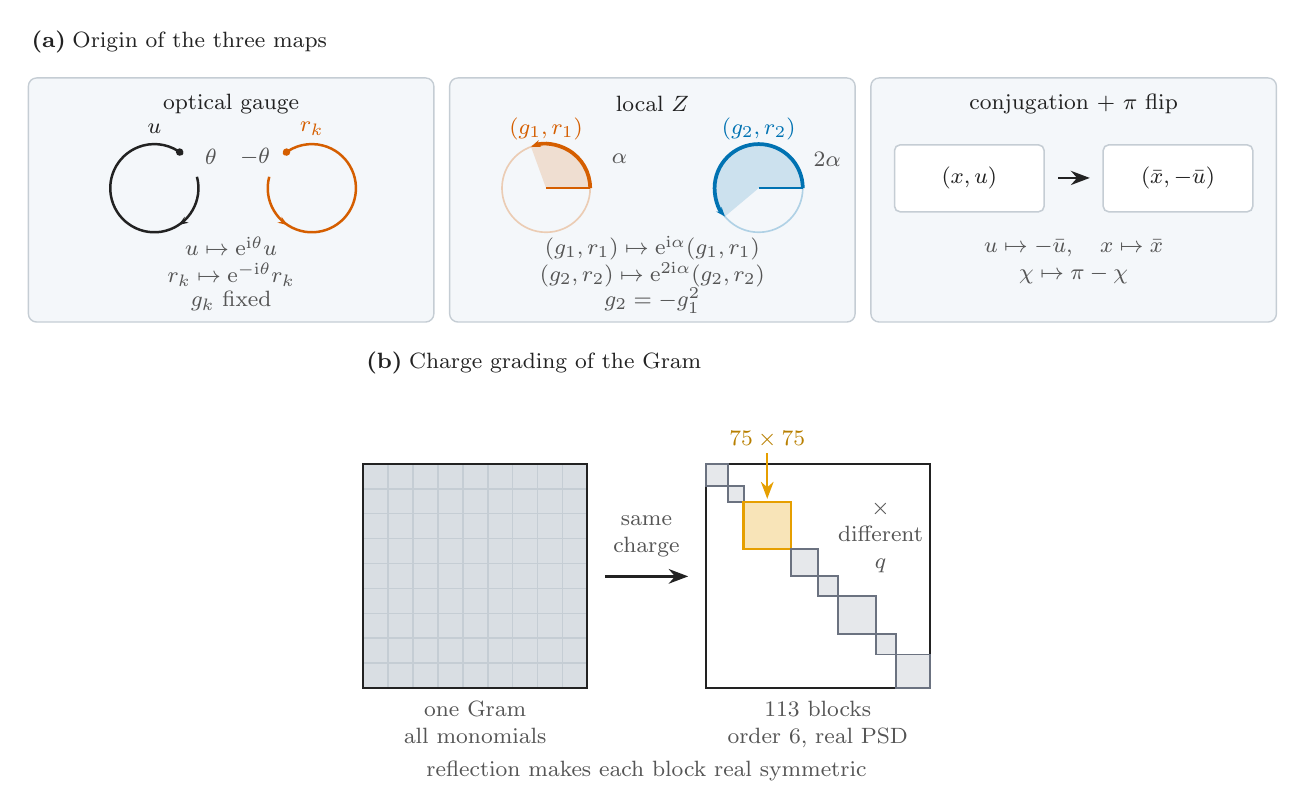
\begin{tikzpicture}[
  x=1cm, y=1cm,
  font=\fontsize{8}{10}\selectfont,
  >=Stealth,
  every node/.append style={inner sep=1pt},
]

% =================================================================
% (a) three origin maps
% =================================================================
\begin{scope}[local bounding box=A]

% --- optical gauge ---
\begin{scope}[local bounding box=A1]
  \draw[boxedge, fill=boxfill, rounded corners=3pt, line width=0.5pt]
    (0.10,5.25) rectangle (5.25,8.35);

  \node[text=ink] at (2.675,8.02) {optical gauge};

  % u circle, CCW by θ
  \draw[ink, line width=0.90pt,
    decoration={markings,
      mark=at position 0.22 with {\arrow{Stealth[length=3.4pt]}}},
    postaction=decorate]
    ([shift={(1.70,6.95)}] 15:0.56) arc[start angle=15, end angle=-310, radius=0.56];
  \fill[ink] ([shift={(1.70,6.95)}] 55:0.56) circle (1.35pt);
  \node[text=ink] at (1.70,7.70) {$u$};
  \node[text=muted] at (2.42,7.35) {$\theta$};

  % r_k circle, CW by −θ
  \draw[brownpop, line width=0.90pt,
    decoration={markings,
      mark=at position 0.22 with {\arrow{Stealth[length=3.4pt]}}},
    postaction=decorate]
    ([shift={(3.70,6.95)}] 165:0.56) arc[start angle=165, end angle=490, radius=0.56];
  \fill[brownpop] ([shift={(3.70,6.95)}] 125:0.56) circle (1.35pt);
  \node[text=brownpop] at (3.70,7.70) {$r_k$};
  \node[text=muted] at (2.98,7.35) {$-\theta$};

  \node[text=muted, align=center] at (2.675,6.02)
    {$u\mapsto\ee^{\ii\theta}u$\\[-0.4pt]
     $r_k\mapsto\ee^{-\ii\theta}r_k$};
  \node[text=muted] at (2.675,5.52) {$g_k$ fixed};
\end{scope}

% --- local Z ---
\begin{scope}[local bounding box=A2]
  \draw[boxedge, fill=boxfill, rounded corners=3pt, line width=0.5pt]
    (5.45,5.25) rectangle (10.60,8.35);

  \node[text=ink] at (8.025,8.02) {local $Z$};

  % sector 1: pie of α (same start ray as sector 2)
  \fill[brownpop, opacity=0.16]
    (8.025-1.35,6.95) -- ++(0:0.56)
    arc[start angle=0, end angle=110, radius=0.56] -- cycle;
  \draw[brownpop, opacity=0.28, line width=0.6pt]
    (8.025-1.35,6.95) circle (0.56);
  \draw[brownpop, line width=0.55pt]
    (8.025-1.35,6.95) -- ++(0:0.56);
  \draw[brownpop, line width=1.35pt, -{Stealth[length=3.4pt]}]
    ([shift={(8.025-1.35,6.95)}] 0:0.56)
    arc[start angle=0, end angle=110, radius=0.56];
  \node[text=brownpop] at (8.025-1.35,7.70) {$(g_1,r_1)$};
  \node[text=muted] at (8.025-0.42,7.32) {$\alpha$};

  % sector 2: pie of 2α
  \fill[tealpop, opacity=0.16]
    (8.025+1.35,6.95) -- ++(0:0.56)
    arc[start angle=0, end angle=220, radius=0.56] -- cycle;
  \draw[tealpop, opacity=0.28, line width=0.6pt]
    (8.025+1.35,6.95) circle (0.56);
  \draw[tealpop, line width=0.55pt]
    (8.025+1.35,6.95) -- ++(0:0.56);
  \draw[tealpop, line width=1.35pt, -{Stealth[length=3.4pt]}]
    ([shift={(8.025+1.35,6.95)}] 0:0.56)
    arc[start angle=0, end angle=220, radius=0.56];
  \node[text=tealpop] at (8.025+1.35,7.70) {$(g_2,r_2)$};
  \node[text=muted] at (8.025+2.22,7.32) {$2\alpha$};

  \node[text=muted, align=center] at (8.025,6.02)
    {$(g_1,r_1)\mapsto\ee^{\ii\alpha}(g_1,r_1)$\\[-0.4pt]
     $(g_2,r_2)\mapsto\ee^{2\ii\alpha}(g_2,r_2)$};
  \node[text=muted] at (8.025,5.52) {$g_2=-g_1^2$};
\end{scope}

% --- conjugation + π flip ---
\begin{scope}[local bounding box=A3]
  \draw[boxedge, fill=boxfill, rounded corners=3pt, line width=0.5pt]
    (10.80,5.25) rectangle (15.95,8.35);

  \node[text=ink] at (13.375,8.02) {conjugation $+\ \pi$ flip};

  \draw[boxedge, fill=white, rounded corners=2pt, line width=0.55pt]
    (11.10,6.65) rectangle (13.00,7.50);
  \node[text=ink] at (12.05,7.08) {$(x,u)$};

  \draw[ink, line width=0.85pt, ->]
    (13.18,7.08) -- (13.58,7.08);

  \draw[boxedge, fill=white, rounded corners=2pt, line width=0.55pt]
    (13.75,6.65) rectangle (15.65,7.50);
  \node[text=ink] at (14.70,7.08) {$(\bar x,-\bar u)$};

  \node[text=muted, align=center] at (13.375,6.02)
    {$u\mapsto-\bar u,\quad x\mapsto\bar x$\\[-0.4pt]
     $\chi\mapsto\pi-\chi$};
\end{scope}

\end{scope}

\node[anchor=south west, font=\fontsize{8}{9.6}\selectfont, text=ink]
  at ($(A.north west)+(0,0.28)$)
  {\textbf{(a)}\;Origin of the three maps};

% =================================================================
% (b) charge grading of the Gram
% =================================================================
\begin{scope}[shift={(4.20,0.05)}, local bounding box=B]
  \def\S{2.85}

  % --- left: one dense Gram ---
  \begin{scope}[shift={(0.15,0.55)}]
    \fill[gramfill] (0,0) rectangle (\S,\S);
    \foreach \i in {1,...,8} {
      \draw[boxedge, line width=0.6pt]
        ({\i*\S/9},0) -- ({\i*\S/9},\S);
      \draw[boxedge, line width=0.6pt]
        (0,{\i*\S/9}) -- (\S,{\i*\S/9});
    }
    \draw[ink, line width=0.7pt] (0,0) rectangle (\S,\S);
    \node[text=muted, align=center, anchor=north]
      at (0.5*\S,-0.12)
      {one Gram\\[-0.2pt]all monomials};
  \end{scope}

  \draw[ink, line width=0.9pt, ->] (3.22,1.97) -- (4.28,1.97);
  \node[text=muted, align=center] at (3.75,2.48) {same\\[-0.2pt]charge};

  % --- right: block-diagonal Gram ---
  \begin{scope}[shift={(4.50,0.55)}]
    \fill[white] (0,0) rectangle (\S,\S);
    \draw[ink, line width=0.7pt] (0,0) rectangle (\S,\S);

    \foreach \ylo/\yhi/\hi in {
      0.00/0.10/0,
      0.10/0.17/0,
      0.17/0.38/1,
      0.38/0.50/0,
      0.50/0.59/0,
      0.59/0.76/0,
      0.76/0.85/0,
      0.85/1.00/0%
    } {
      \ifnum\hi=1
        \fill[patch,opacity=0.28]
          ({\ylo*\S},{\S-\yhi*\S}) rectangle ({\yhi*\S},{\S-\ylo*\S});
        \draw[patch, line width=0.9pt]
          ({\ylo*\S},{\S-\yhi*\S}) rectangle ({\yhi*\S},{\S-\ylo*\S});
      \else
        \fill[blockfill]
          ({\ylo*\S},{\S-\yhi*\S}) rectangle ({\yhi*\S},{\S-\ylo*\S});
        \draw[blockedge, line width=0.7pt]
          ({\ylo*\S},{\S-\yhi*\S}) rectangle ({\yhi*\S},{\S-\ylo*\S});
      \fi
    }

    \node[text=muted] at (0.78*\S,0.80*\S) {$\times$};
    \node[text=muted, align=center] at (0.78*\S,0.62*\S)
      {different\\[-0.2pt]$q$};

    \draw[patch, line width=0.7pt, ->]
      ({0.275*\S},{\S-0.17*\S+0.62}) -- ({0.275*\S},{\S-0.17*\S+0.04});
    \node[text=patch!80!black, anchor=south]
      at ({0.275*\S},{\S-0.17*\S+0.64}) {$75\times75$};

    \node[text=muted, align=center, anchor=north]
      at (0.5*\S,-0.12)
      {$113$ blocks\\[-0.2pt]order $6$, real PSD};
  \end{scope}

  \node[text=muted]
    at (3.75,-0.50)
    {reflection makes each block real symmetric};
\end{scope}

\node[anchor=south west, font=\fontsize{8}{9.6}\selectfont, text=ink]
  at (4.35,4.55)
  {\textbf{(b)}\;Charge grading of the Gram};

\end{tikzpicture}
\end{document}
